\chapter{Proverb 24}

\begin{figure}
  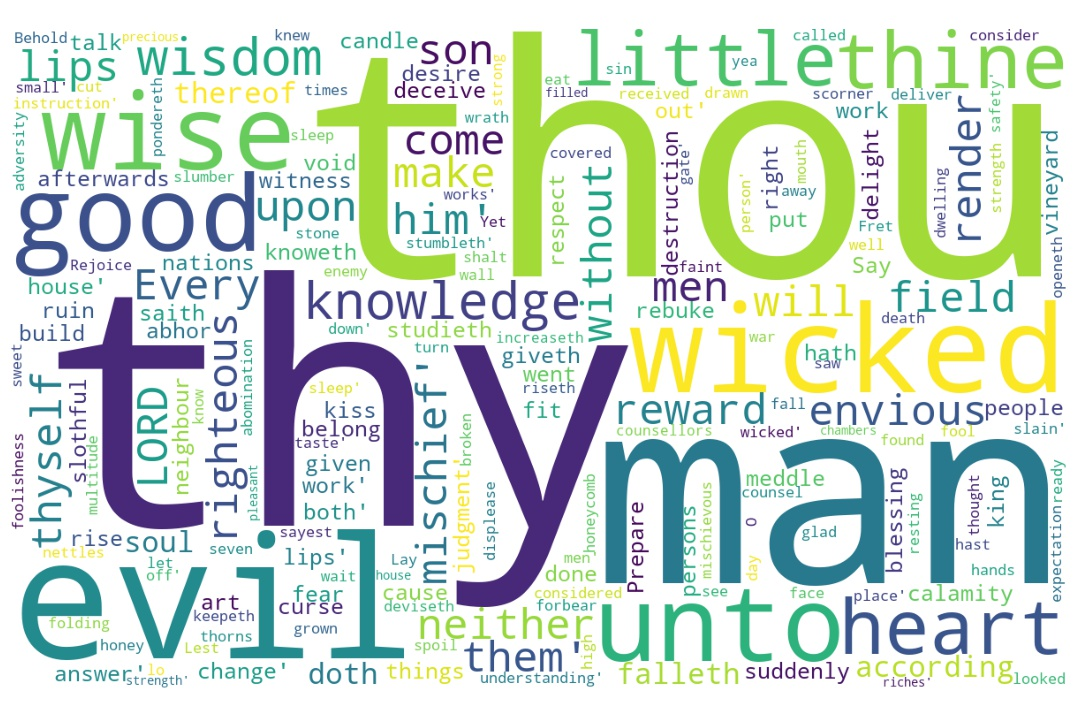
\includegraphics[width=\linewidth]{20OT-Proverbs/Proverb24-WordCloud.jpg}
  \caption{Proverb 24 Word Cloud}
  \label{fig:Proverb 24 word Cloud}
\end{figure}

\marginpar{\scriptsize \centering \fcolorbox{bone}{lime}{\textbf{HOUSE BUILT BY WISDOM}}\\ (Proverb 24:1-5) \begin{compactenum}[I.][8]
    \item \textbf{It is Put Up (Built)} \index[scripture]{Proverbs!Pro 24:03} (Pro 24:3)
    \item \textbf{It is Provided For} \index[scripture]{Proverbs!Pro 24:04} (Pro 24:4)
    \item \textbf{It has Precious Riches} \index[scripture]{Proverbs!Pro 24:04} (Pro 24:4)
    \item \textbf{It is Pleasant} \index[scripture]{Proverbs!Pro 24:04} (Pro 24:4)
    \item \textbf{It is Plenteous} \index[scripture]{Proverbs!Pro 24:04} (Pro 24:4)
    \item \textbf{It is Replete with Goods} \index[scripture]{Proverbs!Pro 24:04} (Pro 24:4)
    \item \textbf{It is Permanent} \index[scripture]{Proverbs!Pro 24:05} (Pro 24:5)
\end{compactenum}}

% \marginpar{\scriptsize \centering \fcolorbox{bone}{yellow}{\textbf{\textcolor[rgb]{1.00,1.00,1.00}{VOID OF UNDERSTANDING}}}\\ (Proverbs 24:1-5) \begin{compactenum}[I.][8]
\marginpar{\scriptsize \centering \fcolorbox{bone}{yellow}{\textbf{VOID OF UNDERSTANDING}}\\ (Proverb 24:1-5) \begin{compactenum}[I.][8]
    \item \textcolor[rgb]{0.00,0.00,0.00}{Is \textbf{Sensual} (\index[scripture]{Proverbs!Pro 7:7}Pro 7:7)}
    \item \textcolor[rgb]{0.00,0.00,0.00}{Reckless \textbf{Speech} (\index[scripture]{Proverbs!Pro 10:13}Pro 10:13)}
    \item \textcolor[rgb]{0.00,0.00,0.00}{Has \textbf{Schemes} (\index[scripture]{Proverbs!Pro 12:11}Pro 12:11)}
    \item \textcolor[rgb]{0.00,0.00,0.00}{Is \textbf{Surety} for Others (\index[scripture]{Proverbs!Pro 17:18}Pro 17:18)}
    \item \textcolor[rgb]{0.00,0.00,0.00}{Is \textbf{Slothful} (\index[scripture]{Proverbs!Pro 24:30}Pro 24:30)}\end{compactenum}}

\marginpar{\scriptsize \centering \fcolorbox{black}{black}{\textbf{\textcolor[rgb]{1.00,1.00,1.00}{THINGS OF THE SLOTHFUL}}}\\ (Proverbs 24:31-33) \begin{compactenum}[I.][8]
    \item \textcolor[rgb]{0.00,0.00,0.00}{His \textbf{Lands} (\index[scripture]{Proverbs!Pro 24:31}Pro 24:31)}
    \item \textcolor[rgb]{0.00,0.00,0.00}{His \textbf{Life} (\index[scripture]{Proverbs!Pro 24:31}Pro 24:31)}
    \item \textcolor[rgb]{0.00,0.00,0.00}{His \textbf{Loves} (\index[scripture]{Proverbs!Pro 24:31}Pro 24:31)}
    \item \textcolor[rgb]{0.00,0.00,0.00}{His \textbf{Learning} (\index[scripture]{Proverbs!Pro 24:31}Pro 24:31)}
    \item \textcolor[rgb]{0.00,0.00,0.00}{His \textbf{Longings} (\index[scripture]{Proverbs!Pro 24:31}Pro 24:31)}
\end{compactenum}}

\marginpar{\scriptsize \centering \fcolorbox{bone}{blue}{\textbf{\textcolor[rgb]{1.00,1.00,1.00}{FIVE JUST MEN}}}\\ (Proverbs 24:16)\\
%\textbf{Introduction:} There are ten references to ``just men'' in scripture. Proverb 9:9 tells us that a just man will listen to instruction and become wiser. Proverb 20:7 tells us that he will maintain integrity. Proverb 24:16 says that, when  he falls, he will get up and get back on the correct path.  Ecclesiastes 7:20 says that just men are difficult to find. Ecclesiastes 7:15 that a just man will go to his grace having nothing but integrity, while a wicked man prolongs his life.
\begin{compactenum}[I.][8]
    \item \textbf{Noah} \index[scripture]{Genesis!Gen 06:09} (Gen 6:9)
    \item \textbf{Joseph} \index[scripture]{Matthew!Mat 01:19} (Mat 1:19)
    \item \textbf{Jesus} \index[scripture]{Matthew!Mat 27:19} (Mat 27:19)
    \item \textbf{John} \index[scripture]{Mark!Mk 06:20} (Mk 6:20)
    \item \textbf{Cornelius} \index[scripture]{Acts!Acts 10:22} (Acts 10:22)
\end{compactenum}}

\footnote{\textcolor[cmyk]{0.99998,1,0,0}{\hyperlink{TOC}{Return to end of Table of Contents.}}}\footnote{\href{https://audiobible.com/bible/proverbs_24.htm}{\textcolor[cmyk]{0.99998,1,0,0}{Proverbs Audio}}}\textcolor[cmyk]{0.99998,1,0,0}{Be not thou envious against evil men, neither desire to be with them.}
[2] \textcolor[cmyk]{0.99998,1,0,0}{For their heart studieth destruction, and their lips talk of mischief.}\footnote{\textbf{Proverbs 15:28} - The heart of the righteous studieth to answer: but the mouth of the wicked poureth out evil things.}
[3] \textcolor[cmyk]{0.99998,1,0,0}{Through wisdom is an house \fcolorbox{bone}{lime}{builded}; and by \fcolorbox{bone}{MYGOLD}{understanding} it is established:}
[4] \textcolor[cmyk]{0.99998,1,0,0}{And by knowledge shall the chambers be \fcolorbox{bone}{lime}{filled} with all \fcolorbox{bone}{lime}{precious} and \fcolorbox{bone}{lime}{pleasant} riches.}
[5] \textcolor[cmyk]{0.99998,1,0,0}{A wise man \emph{is} strong; yea, a man of knowledge \fcolorbox{bone}{lime}{increaseth} strength.}
[6] \textcolor[cmyk]{0.99998,1,0,0}{For by wise counsel thou shalt make thy war: and in multitude of counsellors \emph{there} \emph{is} safety.}
[7] \textcolor[cmyk]{0.99998,1,0,0}{Wisdom \emph{is} too high for a fool: he openeth not his mouth in the gate.}
[8] \textcolor[cmyk]{0.99998,1,0,0}{He that deviseth to do evil shall be called a mischievous person.}\footnote{The connection of the word mischievous is clearly set in scripture in that it is used 5 times, in (1) Psalm 21:11, (2) Psalm 38:12, (3) Proverbs 24:8, (4) Ecclesiastes 10:13, and (5) Micah 7:3. Scripture sets the tone of mischievous as wicked and evil and not ``cute'' as used in the modern context. See, further, the use of the word ``mischief'' as above in verse 2. The word is perhaps best defined by its last use in Acts 13:10: And said, O full of all subtilty and all mischief, thou child of the devil, thou enemy of all righteousness, wilt thou not cease to pervert the right ways of the Lord?}
[9] \textcolor[cmyk]{0.99998,1,0,0}{The thought of foolishness \emph{is} sin: and the scorner \emph{is} an abomination to men.}
[10] \textcolor[cmyk]{0.99998,1,0,0}{\emph{If} thou faint in the day of adversity, thy strength \emph{is} small.}
[11] \textcolor[cmyk]{0.99998,1,0,0}{If thou forbear to deliver \emph{them} \emph{that} \emph{are} drawn unto death, and \emph{those} \emph{that} \emph{are} ready to be slain;}
[12] \textcolor[cmyk]{0.99998,1,0,0}{If thou sayest, Behold, we knew it not; doth not he that pondereth the heart consider \emph{it}? and he that keepeth thy soul, doth \emph{not} he know \emph{it}? and shall \emph{not} he render to \emph{every} man according to his works?}\footnote{\textbf{Jeremiah 17:9, 10} - he heart is deceitful above all things, and desperately wicked: who can know it? [10] I the LORD search the heart, I try the reins, even to give every man according to his ways, and according to the fruit of his doings. }\footnote{\textbf{Matthew 16:27} - For the Son of man shall come in the glory of his Father with his angels; and then he shall reward every man according to his works.}\footnote{\textbf{1 Timothy 4:14} - Alexander the coppersmith did me much evil: the Lord reward him according to his works:}\footnote{\textbf{Hebrews 4:12} - For the word of God is quick, and powerful, and sharper than any twoedged sword, piercing even to the dividing asunder of soul and spirit, and of the joints and marrow, and is a discerner of the thoughts and intents of the heart.}
[13] \textcolor[cmyk]{0.99998,1,0,0}{My son, eat thou honey, because \emph{it} \emph{is} good; and the honeycomb, \emph{which} \emph{is} sweet to thy taste:}
[14] \textcolor[cmyk]{0.99998,1,0,0}{So \emph{shall} the knowledge of wisdom \emph{be} unto thy soul: when thou hast found \emph{it}, then there shall be a reward, and thy expectation shall not be cut off.}
[15] \textcolor[cmyk]{0.99998,1,0,0}{Lay not wait, O wicked \emph{man}, against the dwelling of the righteous; spoil not his resting place:}
[16] \textcolor[cmyk]{0.99998,1,0,0}{For a just \emph{man} falleth seven times, and riseth up again: but the wicked shall fall into mischief.}
[17] \textcolor[cmyk]{0.99998,1,0,0}{Rejoice not when thine enemy falleth, and let not thine heart be glad when he stumbleth:}
[18] \textcolor[cmyk]{0.99998,1,0,0}{Lest the LORD see \emph{it}, and it displease him, and he turn away his wrath from him.}
[19] \textcolor[cmyk]{0.99998,1,0,0}{Fret not thyself because of evil \emph{men}, neither be thou envious at the wicked;}
[20] \textcolor[cmyk]{0.99998,1,0,0}{For there shall be no reward to the evil \emph{man}; the candle of the wicked shall be put out.}\footnote{\textbf{Job 21:17} - How oft is the candle of the wicked put out! and how oft cometh their destruction upon them! God distributeth sorrows in his anger.} 
[21] \textcolor[cmyk]{0.99998,1,0,0}{My son, fear thou the LORD and the king: \emph{and} meddle not with them that are given to change:}\footnote{\textbf{Daniel 7:25} - And he shall speak great words against the most High, and shall wear out the saints of the most High, and think to change times and laws: and they shall be given into his hand until a time and times and the dividing of time.}\footnote{\textbf{Malachi 3:6} - For I am the LORD, I change not; therefore ye sons of Jacob are not consumed.}
[22] \textcolor[cmyk]{0.99998,1,0,0}{For their calamity shall rise suddenly; and who knoweth the ruin of them both?}\footnote{\textbf{Obadiah 1:13} - Thou shouldest not have entered into the gate of my people in the day of their calamity; yea, thou shouldest not have looked on their affliction in the day of their calamity, nor have laid hands on their substance in the day of their calamity;}
[23] \textcolor[cmyk]{0.99998,1,0,0}{These \emph{things} also \emph{belong} to the wise. \emph{It} \emph{is} not good to have respect of persons in judgment.}\footnote{\textbf{2 Chronicles 19:7} - Wherefore now let the fear of the LORD be upon you; take heed and do it: for there is no iniquity with the LORD our God, nor respect of persons, nor taking of gifts.}\footnote{\textbf{Romans 2:11} - For there is no respect of persons with God.}\footnote{\textbf{Ephesians 6:9} - And, ye masters, do the same things unto them, forbearing threatening: knowing that your Master also is in heaven; neither is there respect of persons with him.}
[24] \textcolor[cmyk]{0.99998,1,0,0}{He that saith unto the wicked, Thou \emph{art} righteous; him shall the people curse, nations shall abhor him:}\footnote{\textbf{Romans 12:9} - Let love be without dissimulation. Abhor that which is evil; cleave to that which is good.}
[25] \textcolor[cmyk]{0.99998,1,0,0}{But to them that rebuke \emph{him} shall be delight, and a good blessing shall come upon them.}
[26] \textcolor[cmyk]{0.99998,1,0,0}{\emph{Every} \emph{man} shall kiss \emph{his} lips that giveth a right answer.}
[27] \textcolor[cmyk]{0.99998,1,0,0}{Prepare thy work without, and make it fit for thyself in the field; and afterwards build thine house.}
[28] \textcolor[cmyk]{0.99998,1,0,0}{Be not a witness against thy neighbour without cause; and deceive \emph{not} with thy lips.}
[29] \textcolor[cmyk]{0.99998,1,0,0}{Say not, I will do so to him as he hath done to me: I will render to the man according to his work.}
[30] \textcolor[cmyk]{0.99998,1,0,0}{I went by the field of the slothful, and by the vineyard of the man void of \fcolorbox{bone}{MYGOLD}{understanding};}
[31] \textcolor[cmyk]{0.99998,1,0,0}{And, lo, it was all grown over with thorns, \emph{and} nettles had covered the face thereof, and the stone wall thereof was broken down.}\footnote{\textbf{Job 30:7} - Among the bushes they brayed; under the nettles they were gathered together.}\footnote{\textbf{Isaiah 34:13} - And thorns shall come up in her palaces, nettles and brambles in the fortresses thereof: and it shall be an habitation of dragons, and a court for owls.}\footnote{\textbf{Hosea 9:6} - For, lo, they are gone because of destruction: Egypt shall gather them up, Memphis shall bury them: the pleasant places for their silver, nettles shall possess them: thorns shall be in their tabernacles.}\footnote{\textbf{Zephaniah 2:9} - Therefore as I live, saith the LORD of hosts, the God of Israel, Surely Moab shall be as Sodom, and the children of Ammon as Gomorrah, even the breeding of nettles, and saltpits, and a perpetual desolation: the residue of my people shall spoil them, and the remnant of my people shall possess them. }
[32] \textcolor[cmyk]{0.99998,1,0,0}{Then I saw, \emph{and} considered \emph{it} well: I looked upon \emph{it,} \emph{and} received instruction.}
[33] \textcolor[cmyk]{0.99998,1,0,0}{\emph{Yet} a little sleep, a little slumber, a little folding of the hands to sleep:}
[34] \textcolor[cmyk]{0.99998,1,0,0}{So shall thy poverty come \emph{as} one that travelleth; and thy want as an armed man.}



